\newpage
\section{Morfeas System configuration} \label{sys_conf}
The ``Morfeas System configuration" utility can be accessed from the Morfeas WEB front page from the button with the Morfeas core configuration logo
(
\includegraphics[height=.150in]{../art/morfeas_gear.png}).\\

The 

\begin{figure}[h]
\centering
	\fbox{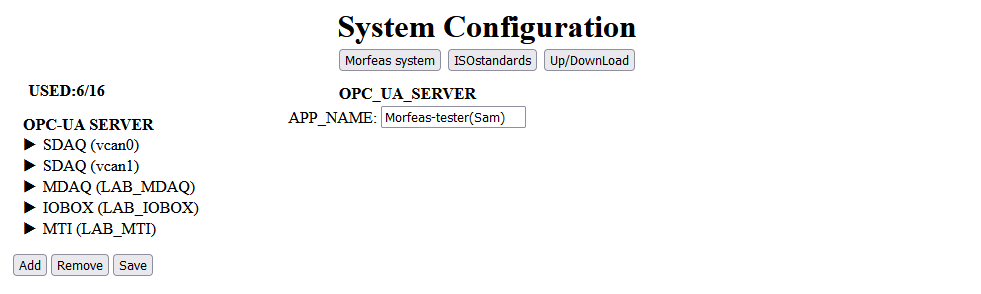
\includegraphics[width=4in,angle=0]{../art/Morfeas_web_if/Morfeas_sys_conf.png}}
	\caption{Morfeas System configuration}
	\label{fig:Morfeas_sys_conf}
\end{figure}

\begin{figure}[h]
\centering
	\fbox{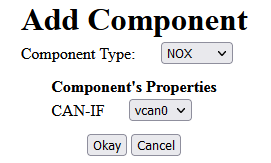
\includegraphics[width=1.5in,angle=0]{../art/Morfeas_web_if/Morfeas_sys_conf_add_comp.png}}
	\caption{Morfeas System add component}
	\label{fig:Morfeas_sys_conf_add_comp}
\end{figure}

\begin{figure}[h]
\centering
	\fbox{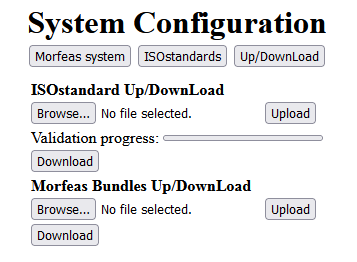
\includegraphics[width=2.5in,angle=0]{../art/Morfeas_web_if/Morfeas_system_conf_up_down.png}}
	\caption{Morfeas System Up/DownLoad}
	\label{fig:sys_conf_up_down}
\end{figure}

\begin{lstlisting}[frame=single,caption=Structure of ISOstandard file,label=lst:ISOStandard]
<?xml version="1.0" encoding="UTF-8"?>
<root>
  <points>
    <ISOStandard_name_tag>
      <description>Description of ISOStandard</description>
      <unit>Default Unit</unit>
      <max>Maximum value</max>
      <min>Minumum value</min>
    </ISOStandard_name_tag>
    ....
  </points>
</root>
\end{lstlisting}